\subsection{Analyze and Visualize User Actions}
The outcome of our reverse engineering challenges is data that describes how each user attacked each obfuscated program in each challenge, and how successful their attack was. Conceptually, our data consists of a list of tuples
\[
    (
    \mathit{user},
    \mathit{challenge},
    \mathit{program},
    \mathit{correctness},
    \mathit{precision},
    \mathit{actions}
    ).
\]
For example, the following user action data
\begin{align}
   &\langle
   (u_0,\mathcal{C}_1,4,
      \mathit{correct},
      0.9,
      \langle a_0,a_1,\ldots\rangle
   ),\\
   &(u_1,\mathcal{C}_3,2,
      \mathit{correct},
      0.7,
      \langle b_0,b_1,\ldots\rangle
   ),
   \ldots
   \rangle
\end{align}
shows that user $u_0$ attempted to reverse engineer the 4th program in challenge $\mathcal{C}_1$ (each challenge contains 10 individual programs to attack, see Section~\ref{sec:generate:program}), our correctness checks indicate that their attack succeeded, the precision of the de-obfuscation was 0.9 (see Section~\ref{sec:precision}), and the user went through the sequence of actions $\langle a_0,a_1,\ldots\rangle$. Each user action $a_i$ is a tuple
\[
    (
    \mathit{time},
    \mathit{kind},
    \mathit{value}
    )
\]
where $\mathit{time}$ is the timestamp when the action was recorded, $\mathit{kind}$ describes the type of data that was collected (such as screenshot, mouse movement, keyboard input, etc.; see Section~\ref{datacollection}), and 
$\mathit{value}$ is the data collected. An example action list might look like this:
\begin{align*}
   \langle 
      &(\mbox{10:23.04},\mathit{screenshot},\mathtt{1.jpg}),\\
      &(\mbox{10:23.05},\mathit{mouseMove},(330,450)),\\
      &(\mbox{10:23.10},\mathit{fileOpen},\mathtt{angr}),
      \ldots
   \rangle
\end{align*}
%In addition to user action data, our database \ also contains demographic information about the users, and responses to the post-attack survey, should the users choose to provide this information.

%%%%%%%%%%%%%%%%%%%%%%%%%%%%%%%%%%%%%%%%%%%%%%
%\begin{figure*}[t]
%\vspace*{-10mm}
%\centering
%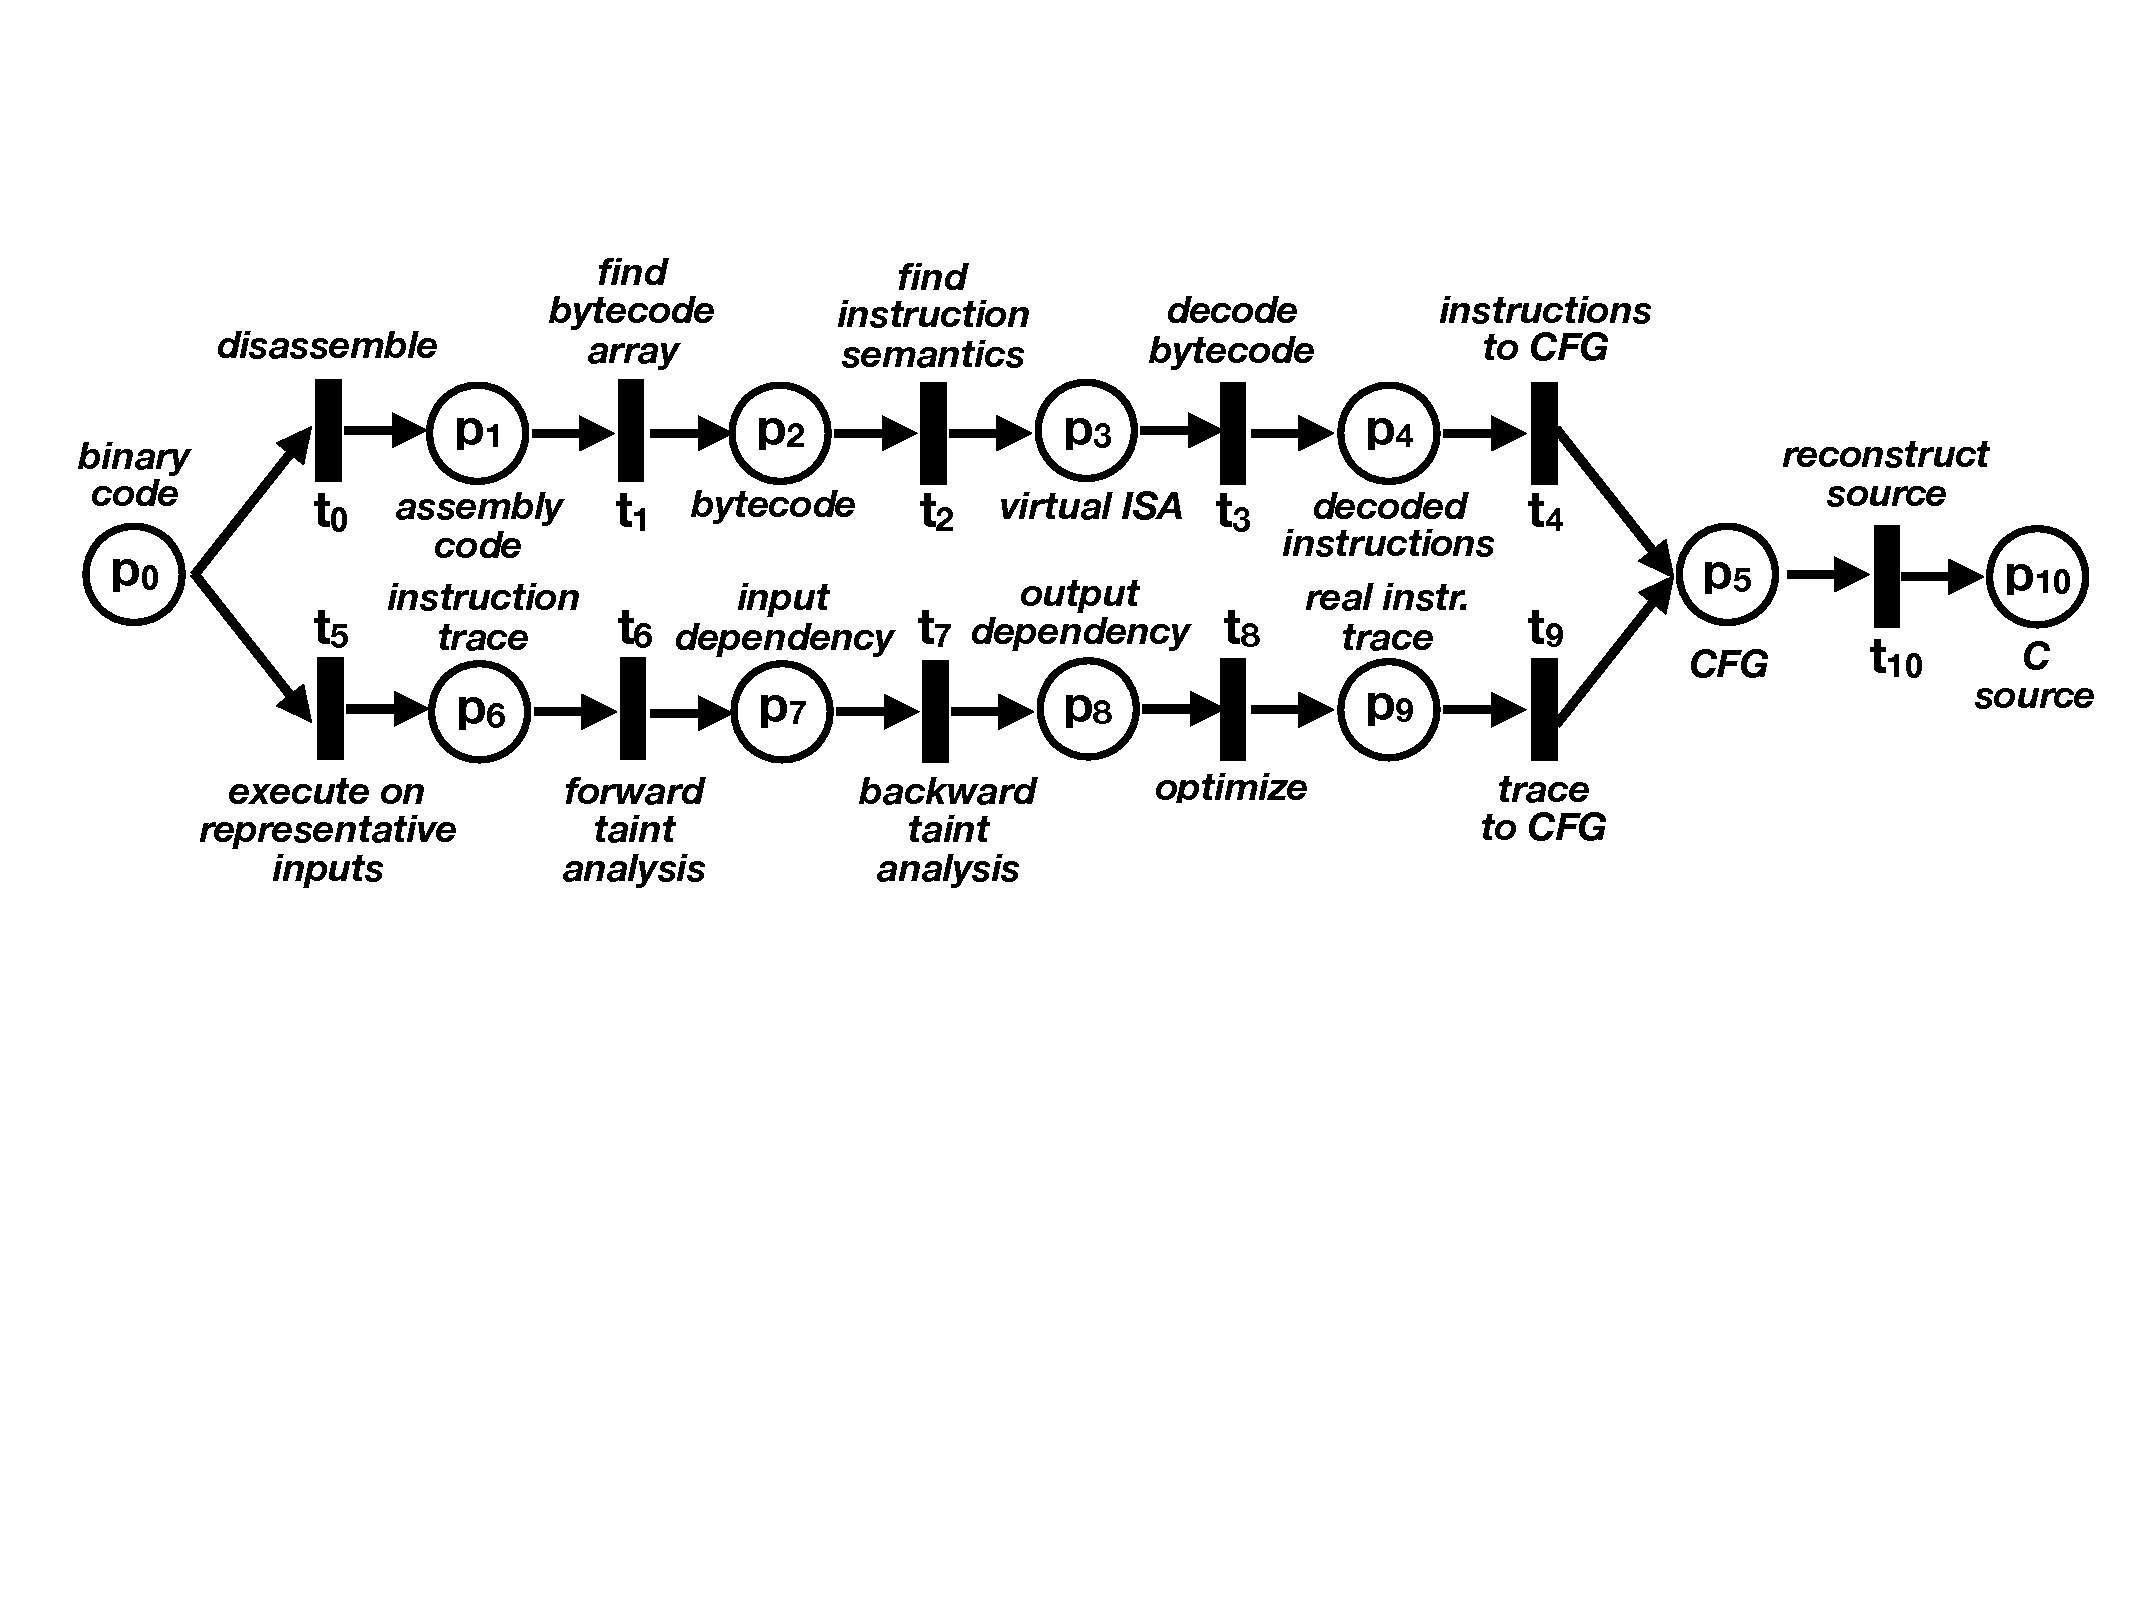
\includegraphics[width=.75\textwidth]{petrivirt.pdf}
%\vspace*{-45mm}
%\caption{Petri net model of two de-virtualization de-obfuscation analyses.}
%\label{fig:petrinet}
%\end{figure*}

\begin{figure}[t]
\vspace*{-10mm}
\hspace*{-8mm}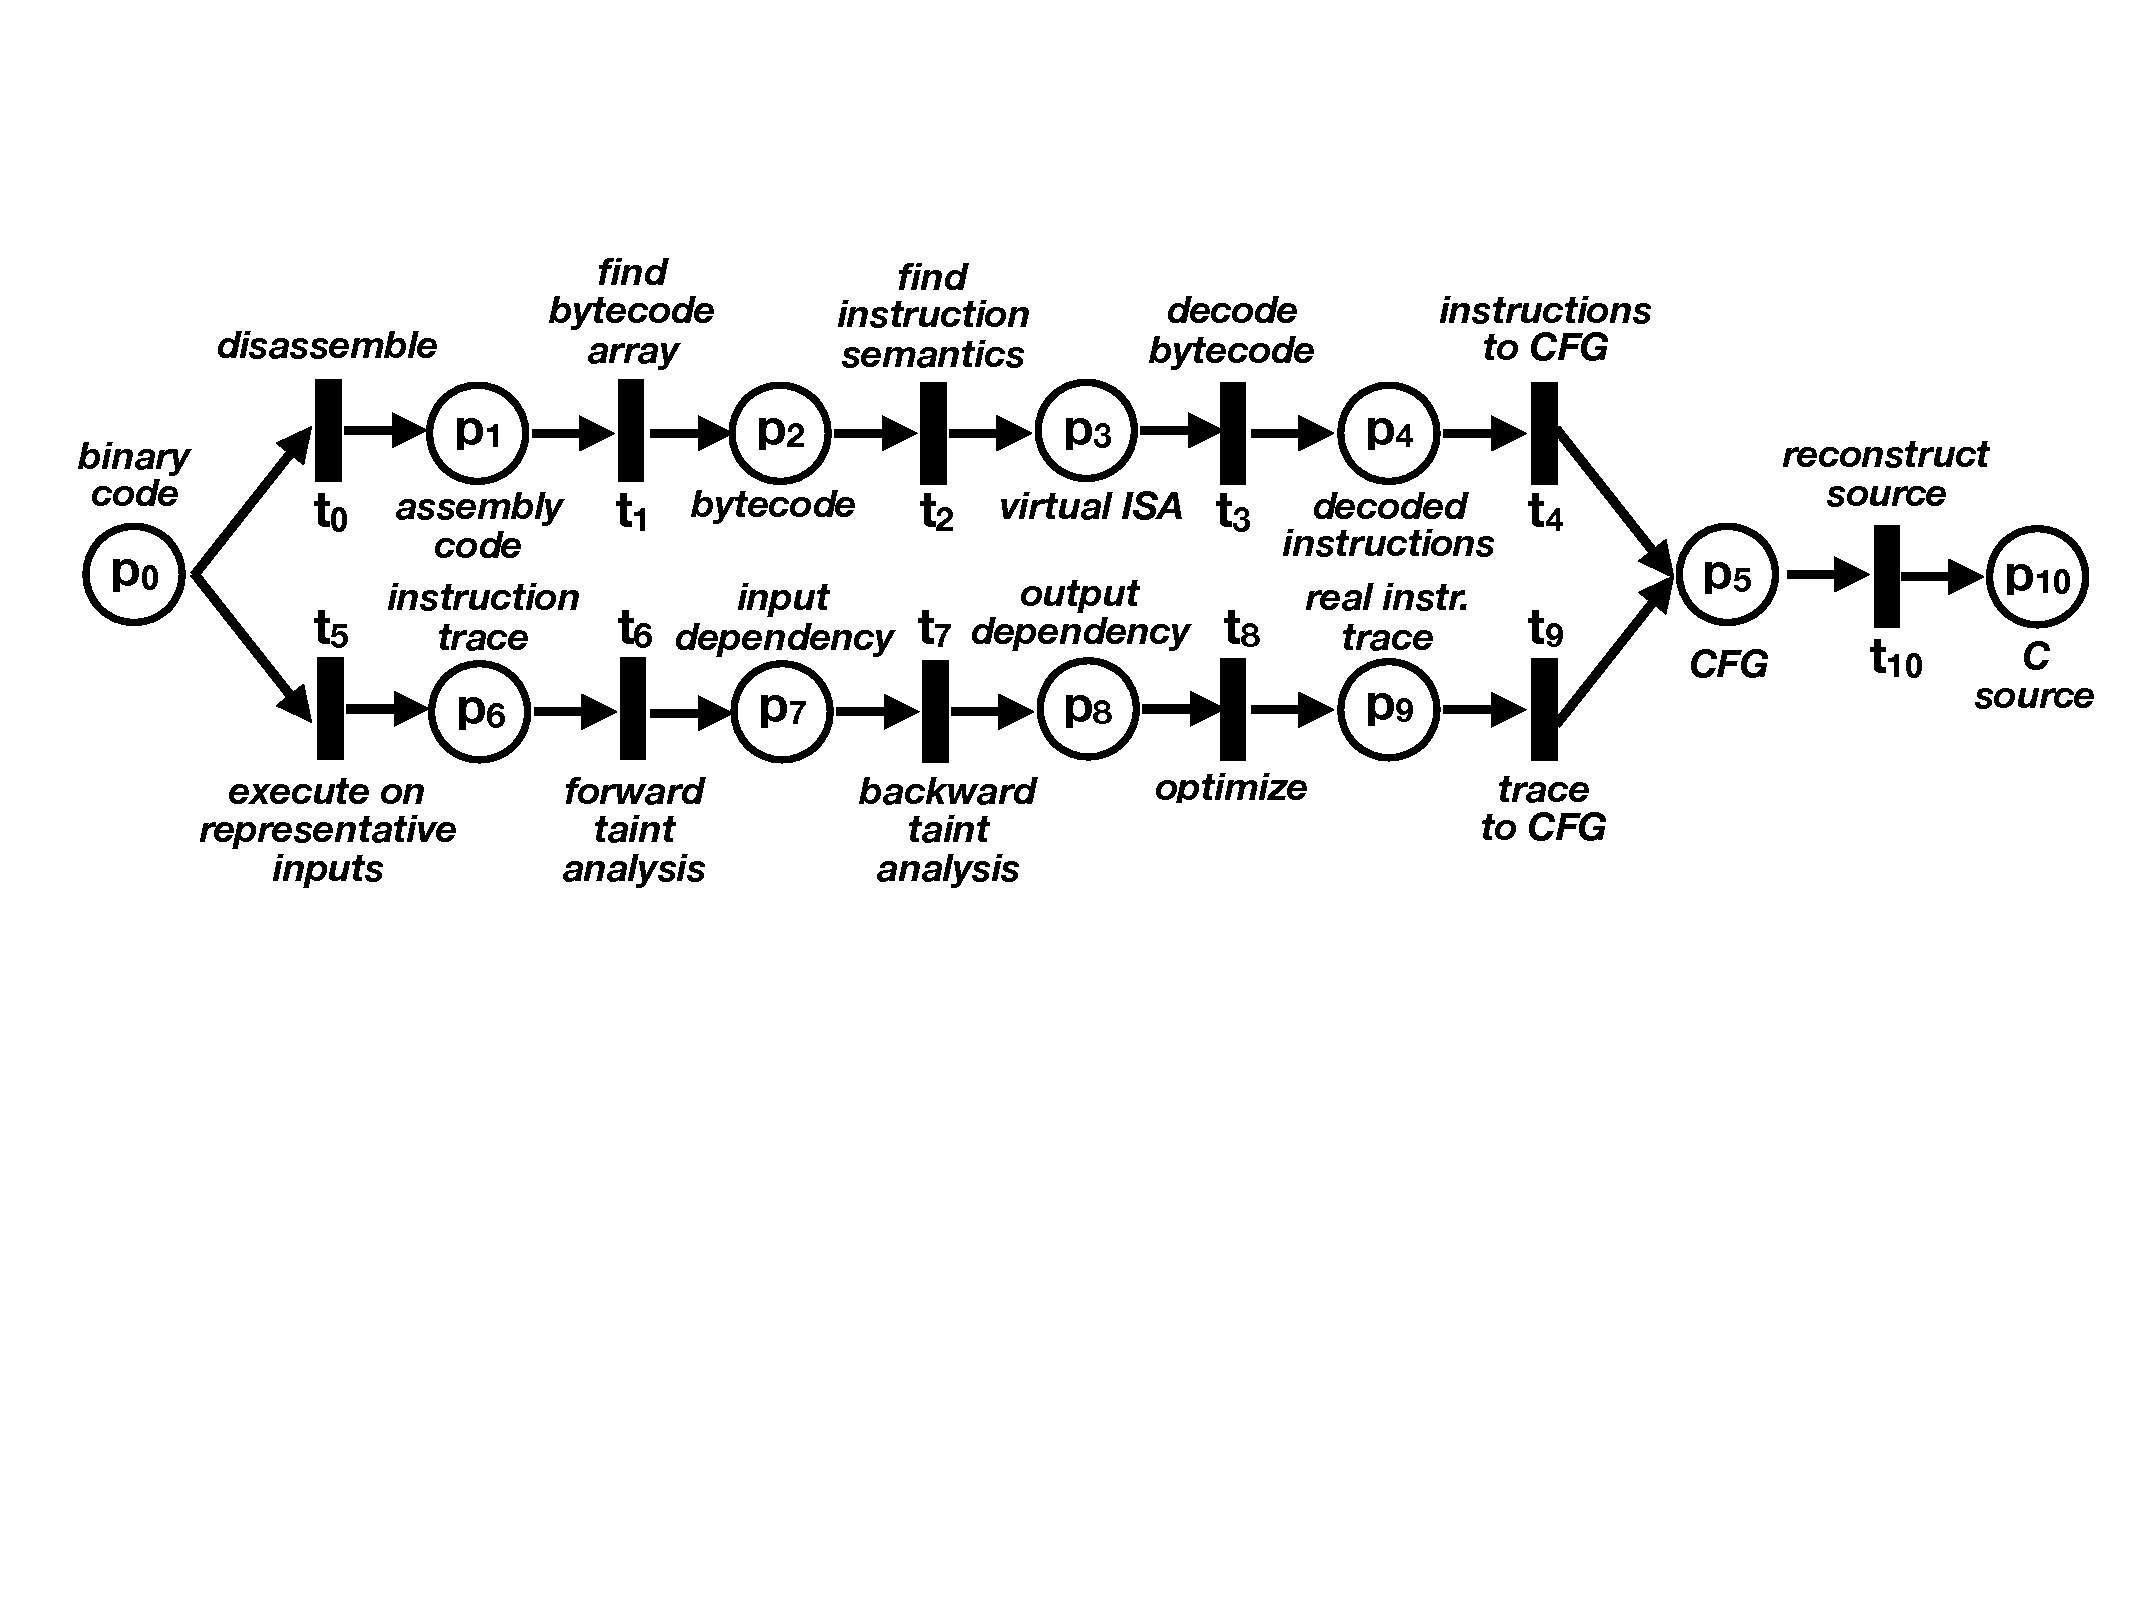
\includegraphics[width=.5\textwidth]{petrivirt.pdf}
\vspace*{-25mm}
\caption{Petri net model of two de-virtualization de-obfuscation analyses.}
\label{fig:petrinet}
\end{figure}

\subsubsection{Building Reverse Engineering Models}
Ultimately, our goal is to be able to extract reverse engineering models from the collected data. While such models have been constructed qualitatively by hand in the past, our data will allow them to be based on the actual actions of reverse engineers in the field.\footnote{Much of the data analysis methodology necessary to fully accomplish this is in progress and constitutes future work.}

Common graphical ways to model attacks are {\em attack trees} and {\em Petri nets}~\cite{su2018method, zhang2016attack, basile2019meta,Wang2013}. As an example, consider Figure~\ref{fig:petrinet} which shows a Petri net modeling two types of attack on virtualized code.
The top path 
\[\langle p_0,t_0,p_1\ldots,t_4,p_5,t_{10},p_{10}\rangle
\]
represents the {\em static analysis} proposed by Rolles~\cite{rolles09unpacking} and the lower path 
\[\langle p_0,t_5,p_6\ldots,t_9,p_5,t_{10},p_{10}\rangle
\]
represents the {\em dynamic analysis} proposed by Yadegari et al.~\cite{yadegari15symbolic}. The $t_i$ are {\em transitions}, actions performed by reverse engineers, and the $p_i$ are {\em states}. A successful attack is a path from $p_0$ to the terminal state, in this case $p_{10}$, which represents the acquisition of de-obfuscated source code. 

%In a typical attack scenario a reverse engineer will explore this graph of potentially successful attack strategies, starting with paths that are {\em cheap} (easy to carry out, requiring few computational resources, etc.) or have a high likelihood of success, backtracking in the graph and reverting to more {\em expensive} strategies when the cheap ones fail. For example, an attacker may attempt the path $\langle p_0,t_0,p_1\ldots,p_{10}\rangle$ first, since a static attack is often easier to carry out. If the virtual instruction set is simple, the attack is likely to work. But, if it is too hard to manually extract the instruction semantics, the attacker might give up on that path, backtrack, and attempt the path $\langle p_0,t_5,p_6\ldots,p_{10}\rangle
%$.

Thus, an attack Petri net is a 6-tuple~\cite{Wang2013} 
\[
  (\mathit{states},
  \mathit{transitions},
  \mathit{arcs},
  \mathit{paths},
  \mathit{rate},
  \mathit{cost}
  )
\]
where $\mathit{rate}$ represents the rate of attack progress, and $\mathit{cost}(t_i)$ represents the cost (to the attacker) of taking a particular transition $t_i$. It is the goal of \revenge to examine the collected data and recover $\mathit{states}$, $\mathit{transitions}$, and
$\mathit{arcs}$ from the sequence of actions that the reverse engineer has performed, and to recover $\mathit{rate}$ and $\mathit{cost}$
by examining the time and memory consumed performing these actions.

%%%%%%%%%%%%%%%%%%%%%%%%%%%%%%%%%%%%%%%%%%%%%%
\begin{figure}[t]
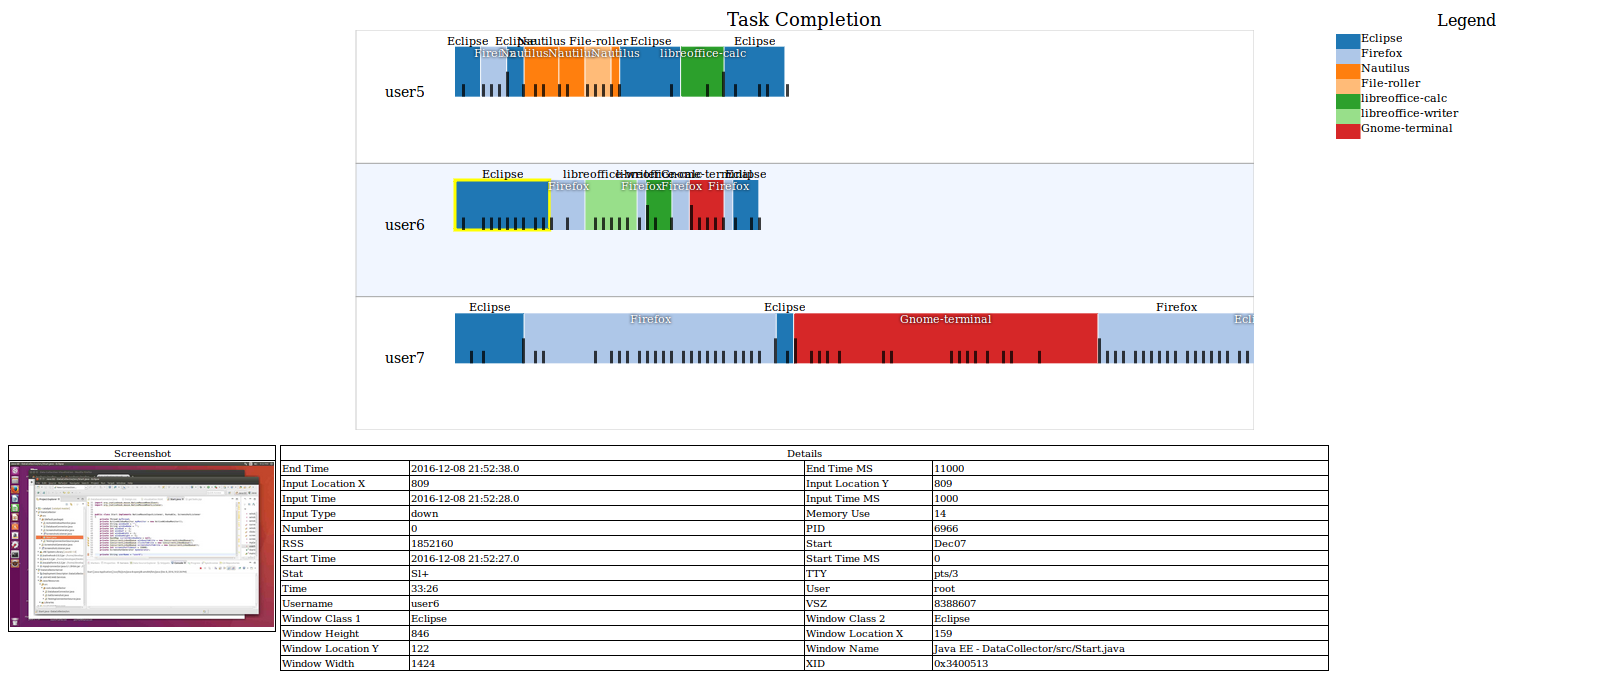
\includegraphics[width=\columnwidth]{screenshot.PNG}
\caption{The visualization component for \revenge's data collection consists of a Gantt chart of in-focus windows and task events per user session; selecting a rectangle shows additional information such as screenshots and the process information.}
\label{fig:screenshot}
\end{figure}

\subsubsection{Visualization of User Actions}
Ultimately, we would like to automatically extract Petri net attack graphs from the collected user action data; doing so requires significant future work in data mining. Initially, however, we have implemented a visualization which will allow us to interactively explore the action events and manually build the attack graph. Figure ~\ref{fig:screenshot} shows the visualization component of \revenge.
Though still in development, the visualization presents events along a Gantt chart timeline with current task information presented below.

%The user-device interaction data contains many dimensions, including in-focus window data,  background program data, keyboard input data, and mouse input data, all of which progress along time and with event tasks.  Within each of these categories, there exist more dimensions: program monitoring, for instance, contains components such as CPU and memory usage.  

%Currently missing in the \revenge visualization is a {\em brushable timeline} which may be used to filter time slots.  Additionally, the visualization will eventually support a suite of sorting and filtering features to narrow down the potentially massive amount of data.  In particular, these sorting and filtering features will allow an analyst to aggregate similar programs and deal with non-typical execution such as running a program through an interpreter, as is the case for Python. In addition, temporal filtering of the timeline will allow zooming for greater detail. 



